\begin{center}
{\Large AudioMouth: Language-Assisted Speech-Driven Mouth Animation with Multimodal Language Models

Supplementary Material}
\end{center}

\section{Dataset Preparation}
\label{app:dataset}

\paragraph{Source Data.}
BEAT~\cite{liu2022beat} contains 76 hours of multimodal recordings from 30 speakers across multiple languages and emotional conditions.
Its facial data comprise 52-dimensional ARKit coefficients captured at 60 Hz with an iPhone 12 Pro, synchronized with 48-kHz stereo audio.
We use its English subset.
% The result tables evaluate 60 scripts; clarify their relation to the 61 test sequences.

\paragraph{Screening.}
We render coefficient sequences with MetaHuman~\cite{metahuman} and manually inspect them together with the synchronized audio.
We discard samples with corrupted or implausible mouth motion, including occlusion-induced tracking failures, or clear audio-motion misalignment.

\paragraph{General and In-the-Wild Recordings.}
The general pipeline uses ASR to obtain transcripts and word-level timestamps, followed by SAT~\cite{frohmann2024segment} for semantic sentence segmentation. The resulting word spans define shared temporal boundaries for the audio and linguistic inputs. Where paired motion is available for training, the same boundaries select the target coefficient subsequences.

\paragraph{Benchmark Inputs.}
The source dataset provides word and phoneme annotations, which we use for the selected data in place of automatically estimated linguistic annotations. Transcript segments are matched to the word intervals in its TextGrid files; the first and last matched words determine each segment's temporal boundaries.
The same interval selects the audio, phonemes, and training coefficient subsequences.
Phonemes come from the provided annotations in all three splits, including testing, and retain CMU ARPAbet lexical stress markers (0/1/2) on vowels.
The segment transcript is constructed from the aligned words.
Target coefficient values provide training supervision and are withheld from the generator at test time.

\section{Additional Implementation Details}
\label{app:implementation}

\subsection{Coefficient Representation and JSON Format}
\label{app:json}

\paragraph{Temporal Resolution and Quantization.}
Following SAiD~\cite{park2023said}, we retain 32 mouth-related ARKit channels.
The preprocessing pipeline converts the original 60-Hz trajectories to 30 Hz by retaining every second frame within each aligned segment.
For a coefficient $v_{t,k}\in[0,1]$, the serialized integer is
\begin{equation}
q_{t,k}=\operatorname{round}(10v_{t,k})\in\{0,1,\ldots,10\}.
\end{equation}
The implementation uses Python's nearest-integer rounding, including ties to even.
Decoded integers are divided by 10 to recover coefficients on the original scale before animation post-processing.

\paragraph{Output Schema.}
Each assistant response is a JSON object with the 32 channel names below, serialized in this order. Each value is an integer array of length $T_j$, ordered chronologically at 30 Hz; every channel in a response has the same length.
The target text uses compact JSON without extra spaces. These strings are processed by the pretrained model's tokenizer.

\begin{center}
\small
\begin{tabular}{r l r l}
\hline
Index & Key & Index & Key \\
\hline
1 & \texttt{JawForward} & 17 & \texttt{MouthStretchRight} \\
2 & \texttt{JawRight} & 18 & \texttt{MouthRollLower} \\
3 & \texttt{JawLeft} & 19 & \texttt{MouthRollUpper} \\
4 & \texttt{JawOpen} & 20 & \texttt{MouthShrugLower} \\
5 & \texttt{MouthClose} & 21 & \texttt{MouthShrugUpper} \\
6 & \texttt{MouthFunnel} & 22 & \texttt{MouthPressLeft} \\
7 & \texttt{MouthPucker} & 23 & \texttt{MouthPressRight} \\
8 & \texttt{MouthRight} & 24 & \texttt{MouthLowerDownLeft} \\
9 & \texttt{MouthLeft} & 25 & \texttt{MouthLowerDownRight} \\
10 & \texttt{MouthSmileLeft} & 26 & \texttt{MouthUpperUpLeft} \\
11 & \texttt{MouthSmileRight} & 27 & \texttt{MouthUpperUpRight} \\
12 & \texttt{MouthFrownLeft} & 28 & \texttt{CheekPuff} \\
13 & \texttt{MouthFrownRight} & 29 & \texttt{CheekSquintLeft} \\
14 & \texttt{MouthDimpleLeft} & 30 & \texttt{CheekSquintRight} \\
15 & \texttt{MouthDimpleRight} & 31 & \texttt{NoseSneerLeft} \\
16 & \texttt{MouthStretchLeft} & 32 & \texttt{NoseSneerRight} \\
\hline
\end{tabular}
\end{center}

For illustration, a three-frame channel entry can be written as \texttt{"JawOpen":[2,4,3]}, corresponding to coefficients $(0.2,0.4,0.3)$. A complete response contains all 32 entries with the same array length.

\paragraph{Model Input and Training Record.}
Each JSONL training record contains a system message specifying the schema and articulation guidance, a user message with the audio placeholder, transcript, phoneme sequence, and requested frame count, and an assistant message containing the coefficient JSON as a string.
The audio file is supplied through the record's audio field.
The requested frame count defines the output duration, while the assistant coefficient sequence is the supervised target.
The articulation guidance connects phoneme groups to named controls, for example bilabial consonants to lip closure and open vowels to jaw opening.

\paragraph{Coefficient-Value Weights.}
The SFT loss uses a fixed lookup table for integers in trajectory arrays:
\begin{equation}
\omega(q)=
\begin{cases}
0.60,&q=0,\\
0.70,&q=1,\\
0.85,&q=2,\\
1.00,&q\in\{3,\ldots,10\}.
\end{cases}
\end{equation}
These are manually specified weights that reduce the contribution of frequent low-valued coefficients. JSON keys and structural punctuation retain unit weight; the reweighting applies only to array-value text.

\subsection{Model Adaptation and Training Configuration}
\label{app:training}

We initialize the generator from Qwen3-Omni-30B-A3B-Instruct~\cite{xu2025qwen3omni} and train with LoRA~\cite{hu2021lora} using four NVIDIA A100 GPUs and BF16 precision.
The audio encoder and multimodal alignment modules remain frozen in both stages.
SFT adapts the decoder's linear layers. GRPO starts from the merged SFT generator and trains new LoRA adapters on the attention query/key/value and output projections.
The two stages use the following settings; batch sizes are global across the training run, rather than per GPU.

\begin{center}
\small
\begin{tabular}{lcc}
\hline
Setting & SFT & GRPO \\
\hline
Epochs & 4 & 4 \\
LoRA rank / $\alpha$ & 32 / 32 & 8 / 16 \\
Micro-batch size & 1 & 1 \\
Global batch size & 8 & 24 \\
Learning rate & $10^{-4}$ & $10^{-6}$ \\
Minimum learning rate & $10^{-5}$ & $10^{-7}$ \\
Warmup fraction & 0.03 & 0.05 \\
Tensor parallel size & 2 & 2 \\
Context parallel size & 2 & 1 \\
Pipeline parallel size & 1 & 1 \\
\hline
\end{tabular}
\end{center}

SFT enables sequence packing with a maximum sequence length of 15,360 tokens.
GRPO permits up to 4,096 prompt tokens and 12,400 completion tokens, uses expert parallel size 4, and clips the gradient norm at 0.5.
% Epochs in both stages follow the authors' confirmed setting; the supplied
% GRPO launcher currently contains a one-epoch setting from another configuration.

\subsection{Sequence-Level Refinement}
\label{app:refinement}

\paragraph{Sampling and Policy Updates.}
GRPO samples $G=6$ candidate sequences per training prompt, with temperature 0.4, top-$p=0.95$, and repetition penalty 1.0.
The training launcher uses one policy-update iteration per sampled group, a policy-ratio clipping parameter of 0.2, and a reference-policy KL coefficient of 0.04.
The KL coefficient controls regularization separately from the four motion-reward weights.
Validation-time sampling uses four candidates per prompt.

\paragraph{Reward Normalization.}
The coefficients and scales in Eqs.~\ref{eq:normalized_score}--\ref{eq:motion_reward} are fixed during refinement:
\begin{center}
\small
\begin{tabular}{lcc}
\hline
Discrepancy & Weight $\lambda_q$ & Scale $s_q$ \\
\hline
Coefficient MSE & 0.30 & 0.660 \\
Velocity & 0.20 & 0.0380 \\
Acceleration & 0.15 & 0.0746 \\
SLMD & 0.35 & 0.0285 \\
\hline
\end{tabular}
\end{center}
The scales are stored reference-median values in the reward implementation.
FD and WInD are not reward terms. Auxiliary diagnostic scores are logged with zero optimization weight.

\paragraph{Validity and Length Handling.}
A candidate must be a parseable JSON object with the expected channels, equally long nonempty arrays, and finite integer values in $[0,10]$.
The reward assigns $-1.5$ to unparseable outputs, $-1.0$ to schema violations, and $-0.8$ to invalid numeric values.
For otherwise valid outputs, let $e_T=|T_p-T_g|/\max(T_g,1)$, where $T_p$ and $T_g$ are the predicted and reference lengths.
Candidates with $e_T>0.20$ receive $-0.6$.
For $e_T\leq0.20$, motion discrepancies are computed on the shared prefix of length $\min(T_p,T_g)$, without interpolation, and the final reward is
\begin{equation}
r=r_{\mathrm{motion}}-0.5\min(e_T,1).
\end{equation}
Thus, shorter or longer valid sequences incur a continuous penalty in addition to their motion error.

\paragraph{Fixed Geometry Asset.}
The SLMD asset is constructed from a neutral mesh and 32 ARKit blendshape meshes with identical topology.
Each basis vector is the displacement from the neutral mesh. The supplied asset retains 606 vertices from a 1,220-vertex mesh, selected using the median of nonzero aggregate deformation magnitudes over the 32 controls.
Fixed spatial weights emphasize the lip region: four nested ellipses in the neutral mesh's frontal plane assign weights of $1.0$, $0.8$, $0.6$, and $0.45$ from the innermost region outward; remaining selected vertices receive $0.1$.
Geometry is measured in the asset's native coordinate units. The basis and weights remain fixed throughout refinement.

\subsection{Inference Post-Processing}
\label{app:postprocessing}

Generated integer trajectories are decoded by dividing by 10 and assembled in temporal order on the recording timeline.
For each coefficient channel, the post-processing pipeline applies dead-zone suppression with threshold 0.02, Gaussian smoothing with standard deviation 1.0 frame and reflected boundaries, and Savitzky--Golay filtering with window length 7 and polynomial order 3.
The Savitzky--Golay filter uses interpolated boundary handling and is applied only when at least seven frames are available.
The final coefficients are clipped to $[0,1]$.

\subsection{Baseline Configuration and Visualization}
\label{app:baselines}

Audio2Face-3D~\cite{chung2025audio2face}, LAM-A2E~\cite{lam}, and SentiAvatar~\cite{jin2026sentiavatar} use publicly released pretrained weights without additional fine-tuning on our dataset.
SAiD~\cite{park2023said} is initialized from its public checkpoint and fine-tuned on our training split.
The comparison uses the mouth-related ARKit channels and speaking intervals described in Section~\ref{sec:experiments}.
Predicted coefficients are rendered with MetaHuman~\cite{metahuman} for qualitative visualization.

\section{Additional Ablation Study}
\label{app:additional_ablation}

\begin{figure}[!htbp]
    \centering
    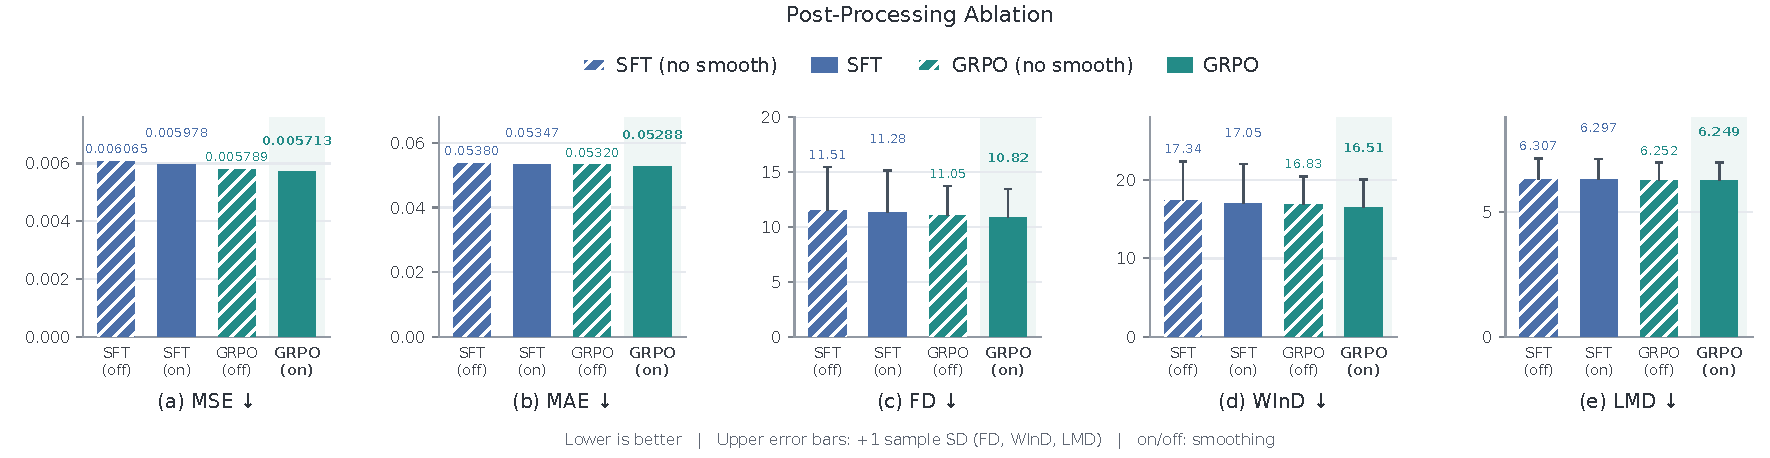
\includegraphics[width=\linewidth]{figures/ablation_smoothing_wide.pdf}
    \caption{Inference-time post-processing for SFT and Refined (GRPO). The labels on/off denote the reported settings with and without smoothing. Results use 60 scripts from the selected test data. SFT is blue and GRPO is teal; hatching identifies the no-smooth variants. Lower values are better. Upper error bars show one sample standard deviation for FD, WInD, and LMD; MSE and MAE are aggregate values.}
    \label{fig:ablation_smoothing}
\end{figure}


\noindent\textbf{Ablation of Inference-Time Post-Processing.}
To distinguish the contribution of post-processing from that of learned motion refinement, we compare SFT and Refined (GRPO) under the reported settings with and without smoothing (Figure~\ref{fig:ablation_smoothing}).
Post-processing produces small improvements across the reported metrics for both generators, while refinement remains beneficial in both settings.
The crossed comparison assesses whether the gains attributed to GRPO persist independently of smoothing.
The filtering operations can suppress local fluctuations and segment-boundary discontinuities, which is consistent with their modest complementary benefit; GRPO instead changes the generator through motion-level feedback during training.
These results support treating post-processing as a complement to motion-aware learning and show that the refinement gains persist without smoothing.

% Original table retained for reference; the figure is used in the compiled manuscript.
% \begin{table}[t]
% \centering
% {\fontsize{9}{10.5}\selectfont
% \renewcommand{\arraystretch}{1.02}
% \begin{tabular*}{\textwidth}{@{\extracolsep{\fill}} lccccc @{}}
% \hline
% \textbf{Methods}
% & \textbf{MSE $\downarrow$}
% & \textbf{MAE $\downarrow$}
% & \textbf{FD $\downarrow$}
% & \textbf{WInD $\downarrow$}
% & \textbf{LMD $\downarrow$} \\
% \hline
%
% SFT (no smooth)
% & $0.006065$
% & $0.053802$
% & $11.510 \pm 3.944$
% & $17.335 \pm 5.017$
% & $6.307 \pm 0.827$ \\
%
% SFT
% & $0.005978$
% & $0.053467$
% & $11.282 \pm 3.888$
% & $17.052 \pm 4.990$
% & $6.297 \pm 0.825$ \\
%
% Refined (no smooth)
% & $0.005789$
% & $0.053197$
% & $11.055 \pm 2.668$
% & $16.830 \pm 3.621$
% & $6.252 \pm 0.716$ \\
%
% Refined (GRPO)
% & $\mathbf{0.005713}$
% & $\mathbf{0.052878}$
% & $\mathbf{10.820 \pm 2.635}$
% & $\mathbf{16.513 \pm 3.584}$
% & $\mathbf{6.249 \pm 0.723}$ \\
% \hline
% \end{tabular*}
% }
% \caption{Training and inference-time post-processing on 60 scripts from the selected test data. ``No smooth'' denotes the reported setting without smoothing. The SFT and Refined (GRPO) rows use the standard post-processing setting. FD, WInD, and LMD are mean $\pm$ sample standard deviation across scripts. Bold marks the lowest reported value in each column.}
% \label{tab:smoothing_ablation}
% \end{table}


\section{Limitations and Future Work}
\label{app:limitations}

\paragraph{Limitations.}
The experiments on the selected data use provided word and phoneme annotations at test time. Performance with automatically recognized phonemes remains to be established. The linguistic inputs and baseline adaptation settings differ across methods, so the benchmark compares their stated configurations rather than isolating architecture alone.
The current scope is limited to 32 mouth-related ARKit coefficients and a fixed geometry basis for reward computation. Autoregressive JSON generation requires a long output sequence, and its latency has not been characterized for real-time deployment.
SLMD remains a surrogate for mouth deformation: although the completed ablation supports its contribution to refinement, it does not establish equivalence to rendered-video LMD. The reported mean differences do not establish statistical significance, and some ablated conditions exhibit substantial variation across scripts. The conditioning ablation tests transcripts and phonemes jointly and does not isolate their individual effects or the shared segmentation stage. The post-processing comparison evaluates the reported pipeline settings rather than isolating each filtering operation.
Moreover, improved facial animation techniques may also be misused for synthetic media generation, highlighting the importance of responsible deployment and appropriate safeguards.
\paragraph{Future Work.}
 
Leveraging the instruction-following ability of MLLMs, we plan to support explicit emotional control through natural language prompts, enabling richer and more expressive facial animations. We will also extend the framework to full-face coefficient generation, develop speaker-adaptive and few-shot personalization techniques, and improve robustness under in-the-wild, multilingual, and noisy conditions.
